\section{Introduction}
In the modern world, the Portable Document Format $-$ PDF format of documents is widely used for sharing and printing documents, because unline other types such as docx, the PDF type does not change the contents and format (layout, font, etc) when we read it on different devices. The scientific documents are no exception. In these documents, mathematical formulas play important parts. As a result, there is a need of a tool that detect these formulas, which is a precondition for reusing these formulas in our own documents. A good example is the preprint repositories \href{arXiv.org}{arXiv.org}, which gives readers access to the \LaTeX source files along with the PDF files, but there is only a small number of the existing PDF documents on this website. We ourselves used to meet difficulties when we tried to re-type math formulas in PDF documents to our ones, therefore we want to build a model that can do the task of mathematical formula detection in PDF documents.

Unlike comment text content, general OCR software fails to detect math formulas. Usually, we have to detect the regions of mathematical formulas in documents. We proposed a model with Faster R-CNN and ResNet50 as the "core" as our solution for this problem.
\begin{figure}[H]
\centering{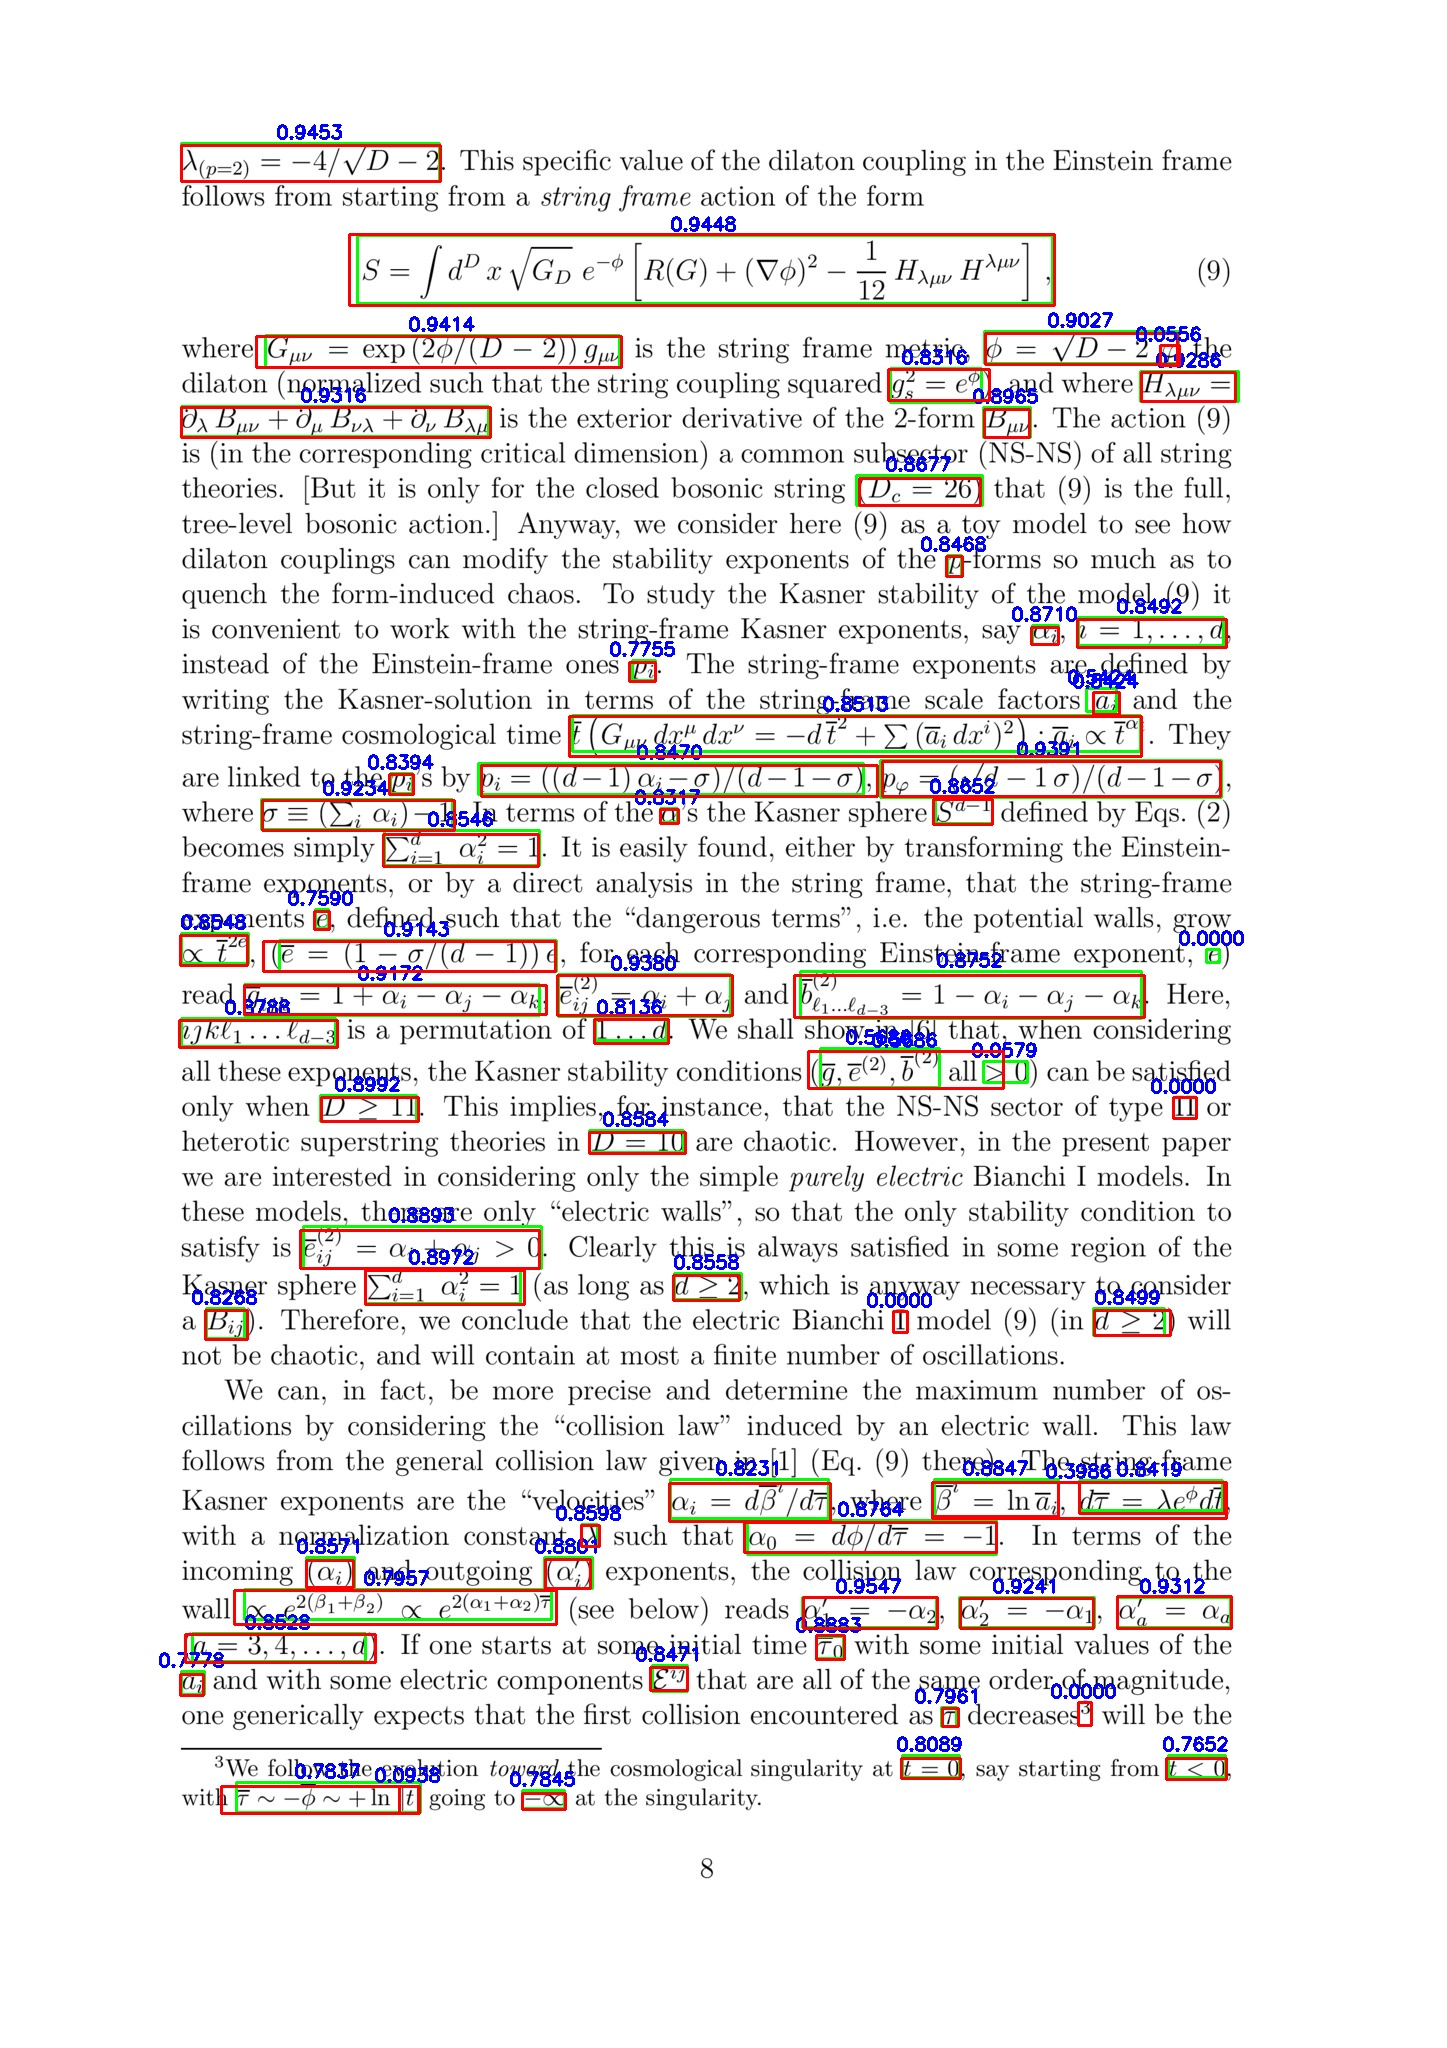
\includegraphics[scale=0.2]{intro/intro.jpg}}
\caption{Detection of mathematical formulas in PDF documents}
\end{figure}
